\documentclass[UTF8,zihao=-4]{ctexart}
\usepackage[a4paper,top=2.0cm,bottom=2.0cm,left=2.2cm,right=2.2cm]{geometry}
\usepackage{booktabs,tabularx,array,float}
\usepackage{graphicx,caption}
\usepackage{xcolor,listings,tcolorbox}
\usepackage{fancyhdr,lastpage}
\usepackage[hidelinks]{hyperref}

\definecolor{navy}{HTML}{183B63}
\definecolor{blue}{HTML}{2B6EAE}
\definecolor{green}{HTML}{2F8F49}
\definecolor{orange}{HTML}{DF7615}
\definecolor{purple}{HTML}{7651B5}
\definecolor{soft}{HTML}{F3F7FB}
\definecolor{line}{HTML}{C9D4DF}
\definecolor{codebg}{HTML}{F6F8FA}
\definecolor{headergray}{HTML}{777777}
\hypersetup{pdftitle={系统开发工具基础 - 第4周实验报告},pdfauthor={朱元清},colorlinks=true,linkcolor=blue,urlcolor=blue}
\pagestyle{fancy}\fancyhf{}
\setlength{\headheight}{24pt}
\fancyhead[L]{\small\color{headergray}系统开发工具基础}
\fancyhead[R]{\small\color{headergray}第 4 周实验报告}
\fancyfoot[C]{\small\color{headergray}第 \thepage\ 页 / 共 \pageref{LastPage} 页}
\renewcommand{\headrulewidth}{0.5pt}
\renewcommand{\headrule}{\hbox to\headwidth{\color{line}\leaders\hrule height \headrulewidth\hfill}}
\lstdefinestyle{shell}{language=bash,basicstyle=\ttfamily\footnotesize,backgroundcolor=\color{codebg},frame=single,rulecolor=\color{line},breaklines=true,columns=fullflexible,keepspaces=true,showstringspaces=false,xleftmargin=.3em,xrightmargin=.3em,aboveskip=.6em,belowskip=.7em}
\newtcolorbox{summarybox}[1]{colback=soft,colframe=blue,boxrule=.7pt,arc=2mm,title={#1},fonttitle=\bfseries,coltitle=navy}
\newcommand{\exercisebanner}[3]{\begin{tcolorbox}[colback=soft,colframe=navy,boxrule=1pt,arc=2mm,left=4mm,right=4mm,top=2.5mm,bottom=2.5mm]\begin{tabularx}{\textwidth}{>{\Large\bfseries\color{navy}}p{2.7cm}X}练习 #1 & {\large\bfseries\color{navy}#2}\quad{\normalsize（#3）}\end{tabularx}\end{tcolorbox}}
\setlength{\parindent}{2em}\setlength{\parskip}{.25em}
\begin{document}
\vspace*{.7cm}\begin{center}
{\fontsize{28}{34}\selectfont\bfseries 系统开发工具基础}\\[.35cm]
{\fontsize{22}{28}\selectfont 第 4 周实验报告}\\[1cm]
{\Large 姓名：朱元清\qquad 学号：25020007193}\\[.6cm]
{\Large 2026 年 9 月 14 日}
\end{center}
\vspace{.7cm}
\begin{tcolorbox}[colback=soft,colframe=navy,boxrule=.8pt,arc=2mm,left=5mm,right=5mm,top=4mm,bottom=4mm]
\centering 本报告记录第 4 周代码质量练习与课堂综合题的实际执行结果。内容覆盖格式化、静态检查、测试、覆盖率、提交前检查、持续集成、命令运行器、正则表达式，以及 q13--q16 的质量门禁、Make 构建、API 报告和软件包交付。
\end{tcolorbox}
\vspace{.55cm}
\begin{table}[H]\centering\caption{第 4 周任务完成情况}\renewcommand{\arraystretch}{1.22}
\begin{tabularx}{.96\textwidth}{cX>{\raggedright\arraybackslash}p{4.1cm}c}\toprule
编号&主题&关键工具&状态\\\midrule
13&建立可执行的本地质量门禁&Ruff、pytest、Shell&完成\\
14&让 Make 只重建受影响的产物&Make、Python&完成\\
15&把本地 API 数据转换为可读报告&curl、jq、Markdown&完成\\
16&修复并交付陌生小型工具包&Make、build、Git&完成\\
1&格式化与只检查模式&Ruff format&完成\\
2&静态检查与自动修复&Ruff check&完成\\
3&单元测试与边界条件&pytest&完成\\
4&覆盖率报告与补测&coverage.py、pytest&完成\\
5&提交前质量门禁&pre-commit&完成\\
6&持续集成工作流&GitHub Actions&完成\\
7&统一命令入口&Make&完成\\
8&查找危险 shell 调用&grep、regex&完成\\
9&Markdown 精确替换&regex&完成\\
10&JSON 名称提取&regex、json&完成\\\bottomrule
\end{tabularx}\end{table}
\clearpage\exercisebanner{13}{建立可执行的本地质量门禁}{Ruff、pytest 与 Shell}
\subsection*{执行内容}
以 q10 的 \texttt{greetlab} 项目为基础，在 q13 中保留 \texttt{src/} 与 \texttt{tests/} 的标准结构，补充 Ruff 和 pytest 配置，并创建 \texttt{check.sh}。脚本依次执行格式检查、静态检查和单元测试；空白姓名应触发 argparse 错误并返回退出码 2。
\begin{lstlisting}[style=shell]
python -m ruff format .
python -m ruff check .
python -m pytest
./check.sh
echo $?
\end{lstlisting}
\begin{figure}[H]\centering
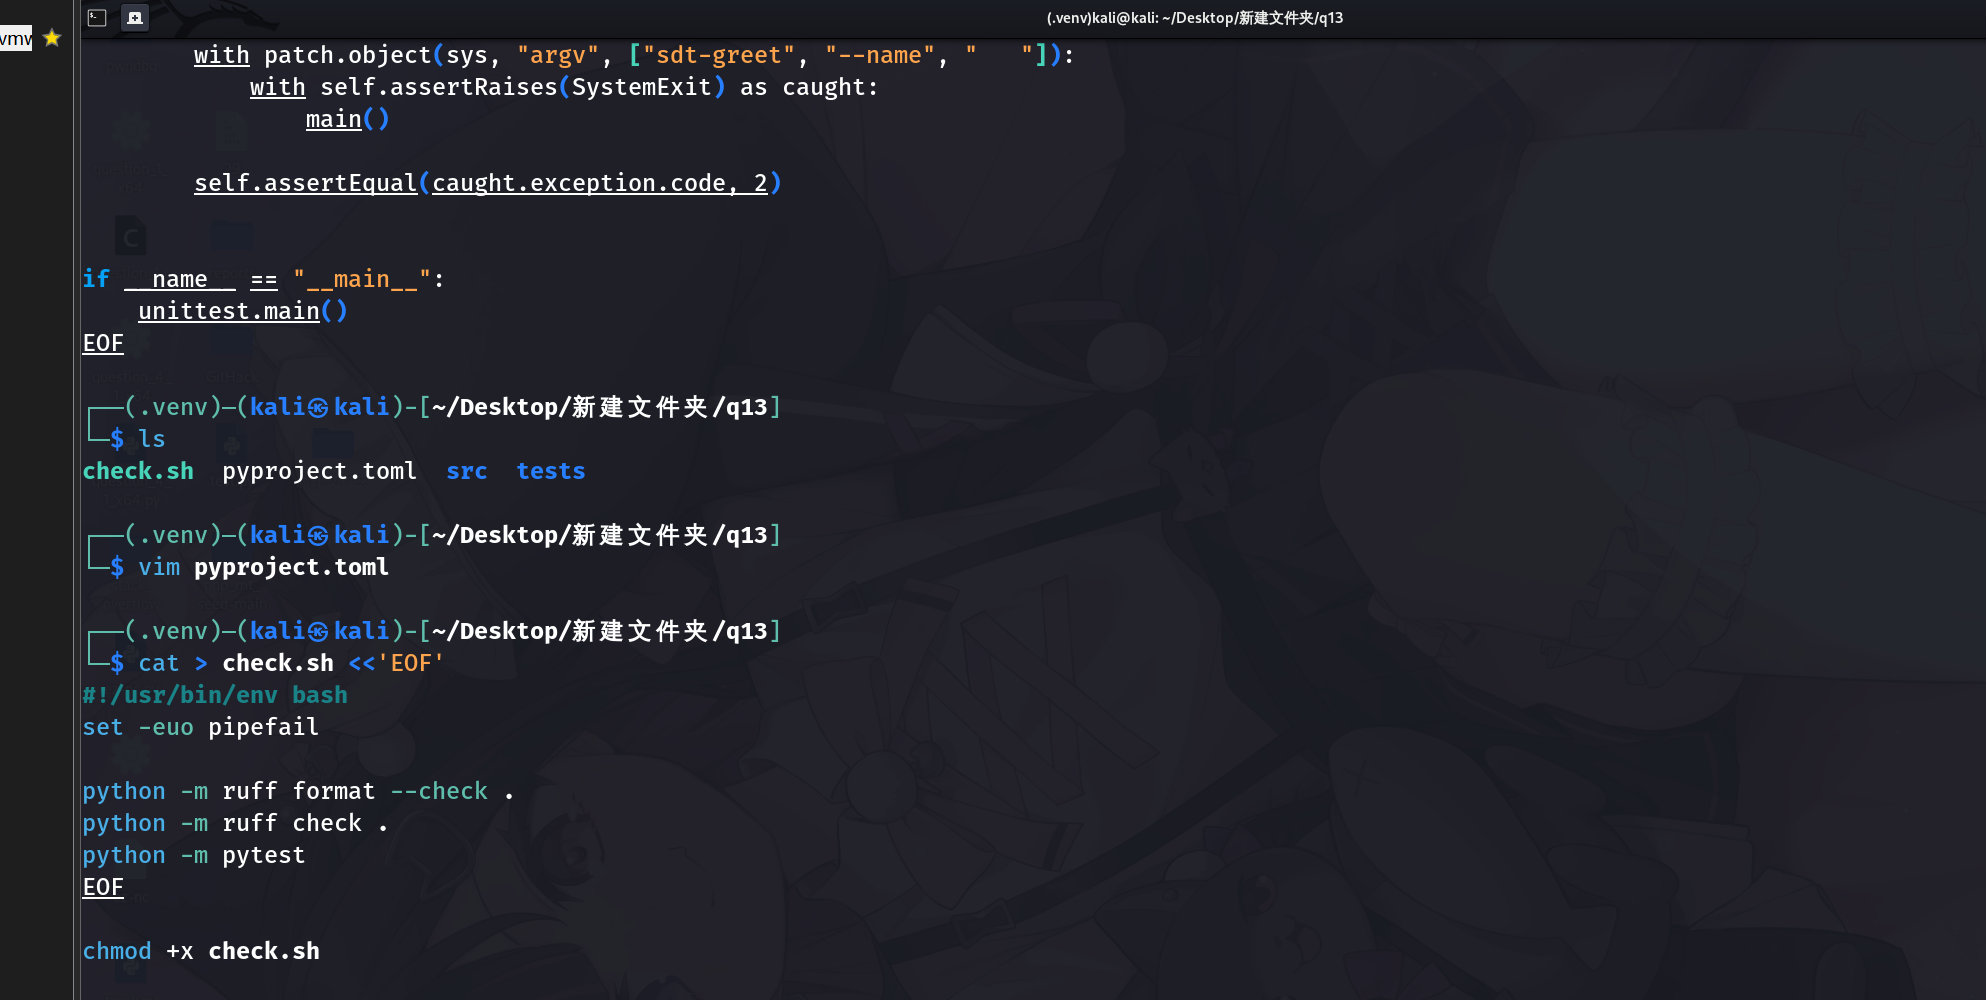
\includegraphics[width=.94\textwidth,height=.35\textheight,keepaspectratio]{assets/q13-setup.png}
\caption{q13 的测试目录与检查脚本配置}
\end{figure}
\begin{figure}[H]\centering
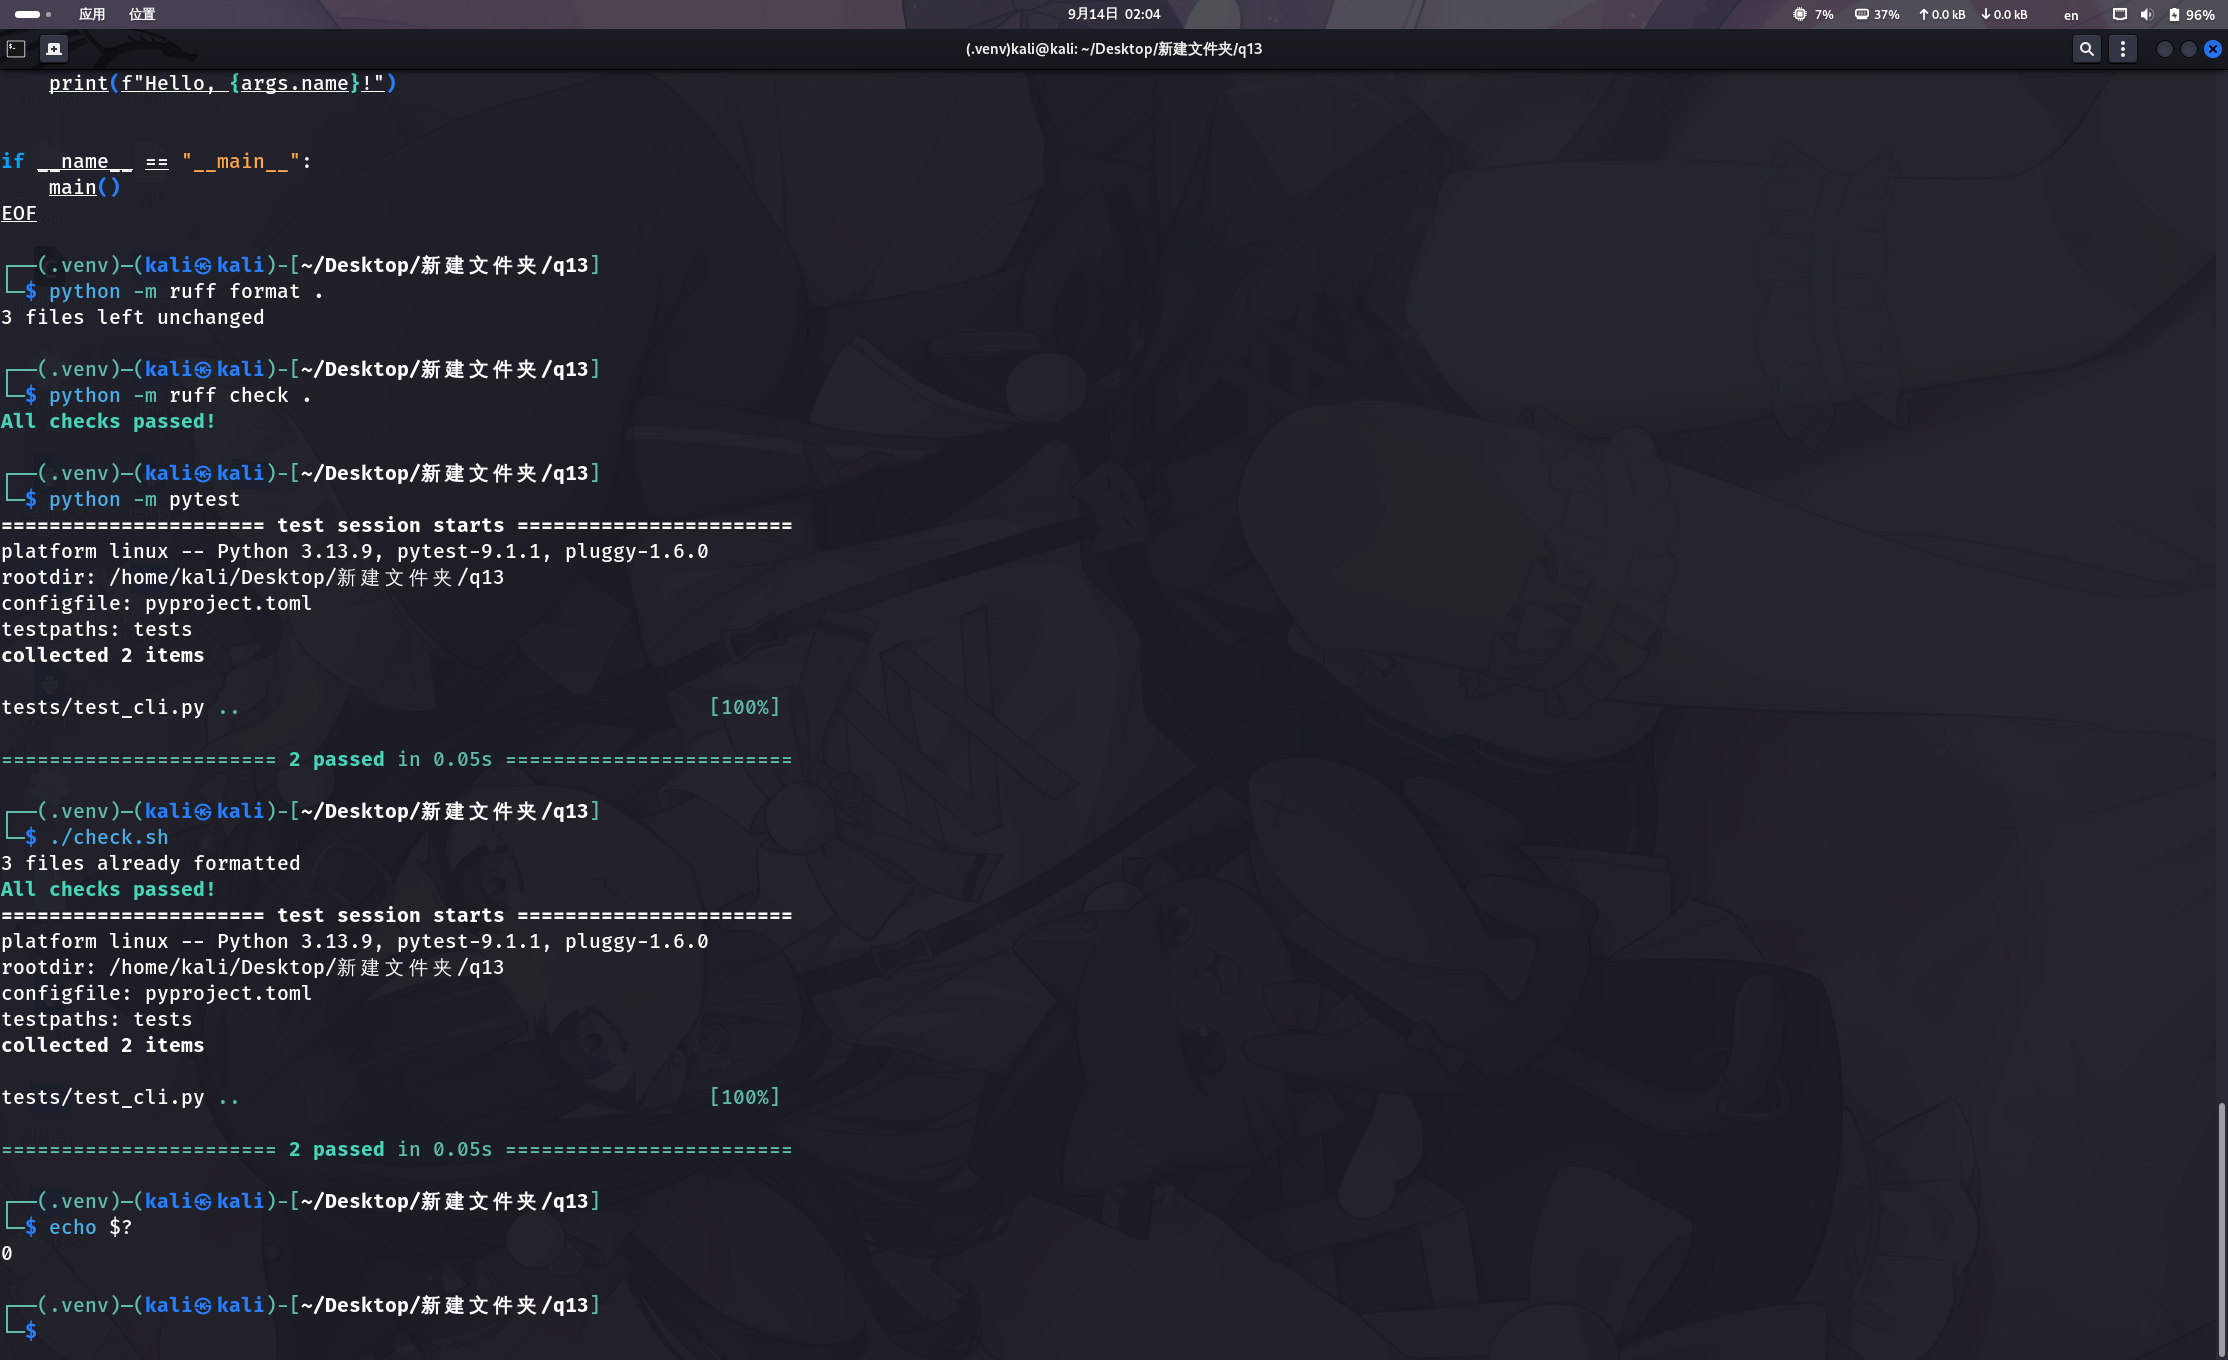
\includegraphics[width=.94\textwidth,height=.36\textheight,keepaspectratio]{assets/q13-check.png}
\caption{q13 格式化、静态检查与两项单元测试均通过}
\end{figure}
\begin{summarybox}{结果说明}Ruff 显示 3 个文件已符合格式，静态检查通过；pytest 收集 2 项测试并全部通过，\texttt{check.sh} 的退出状态为 0。\end{summarybox}

\clearpage\exercisebanner{14}{让 Make 只重建受影响的产物}{Make 依赖关系}
\subsection*{执行内容}
\texttt{stats.txt} 依赖 \texttt{data.csv} 和 \texttt{stats.py}，\texttt{report.txt} 进一步依赖 \texttt{stats.txt}、\texttt{report.md} 与 \texttt{build\_report.py}。首次 \texttt{make} 生成两个产物；随后未修改文件时不执行配方；更新 \texttt{data.csv} 的时间戳后，两项产物重新生成。
\begin{lstlisting}[style=shell]
make
cat stats.txt
cat report.txt
make
touch data.csv
make
make clean
\end{lstlisting}
\begin{figure}[H]\centering
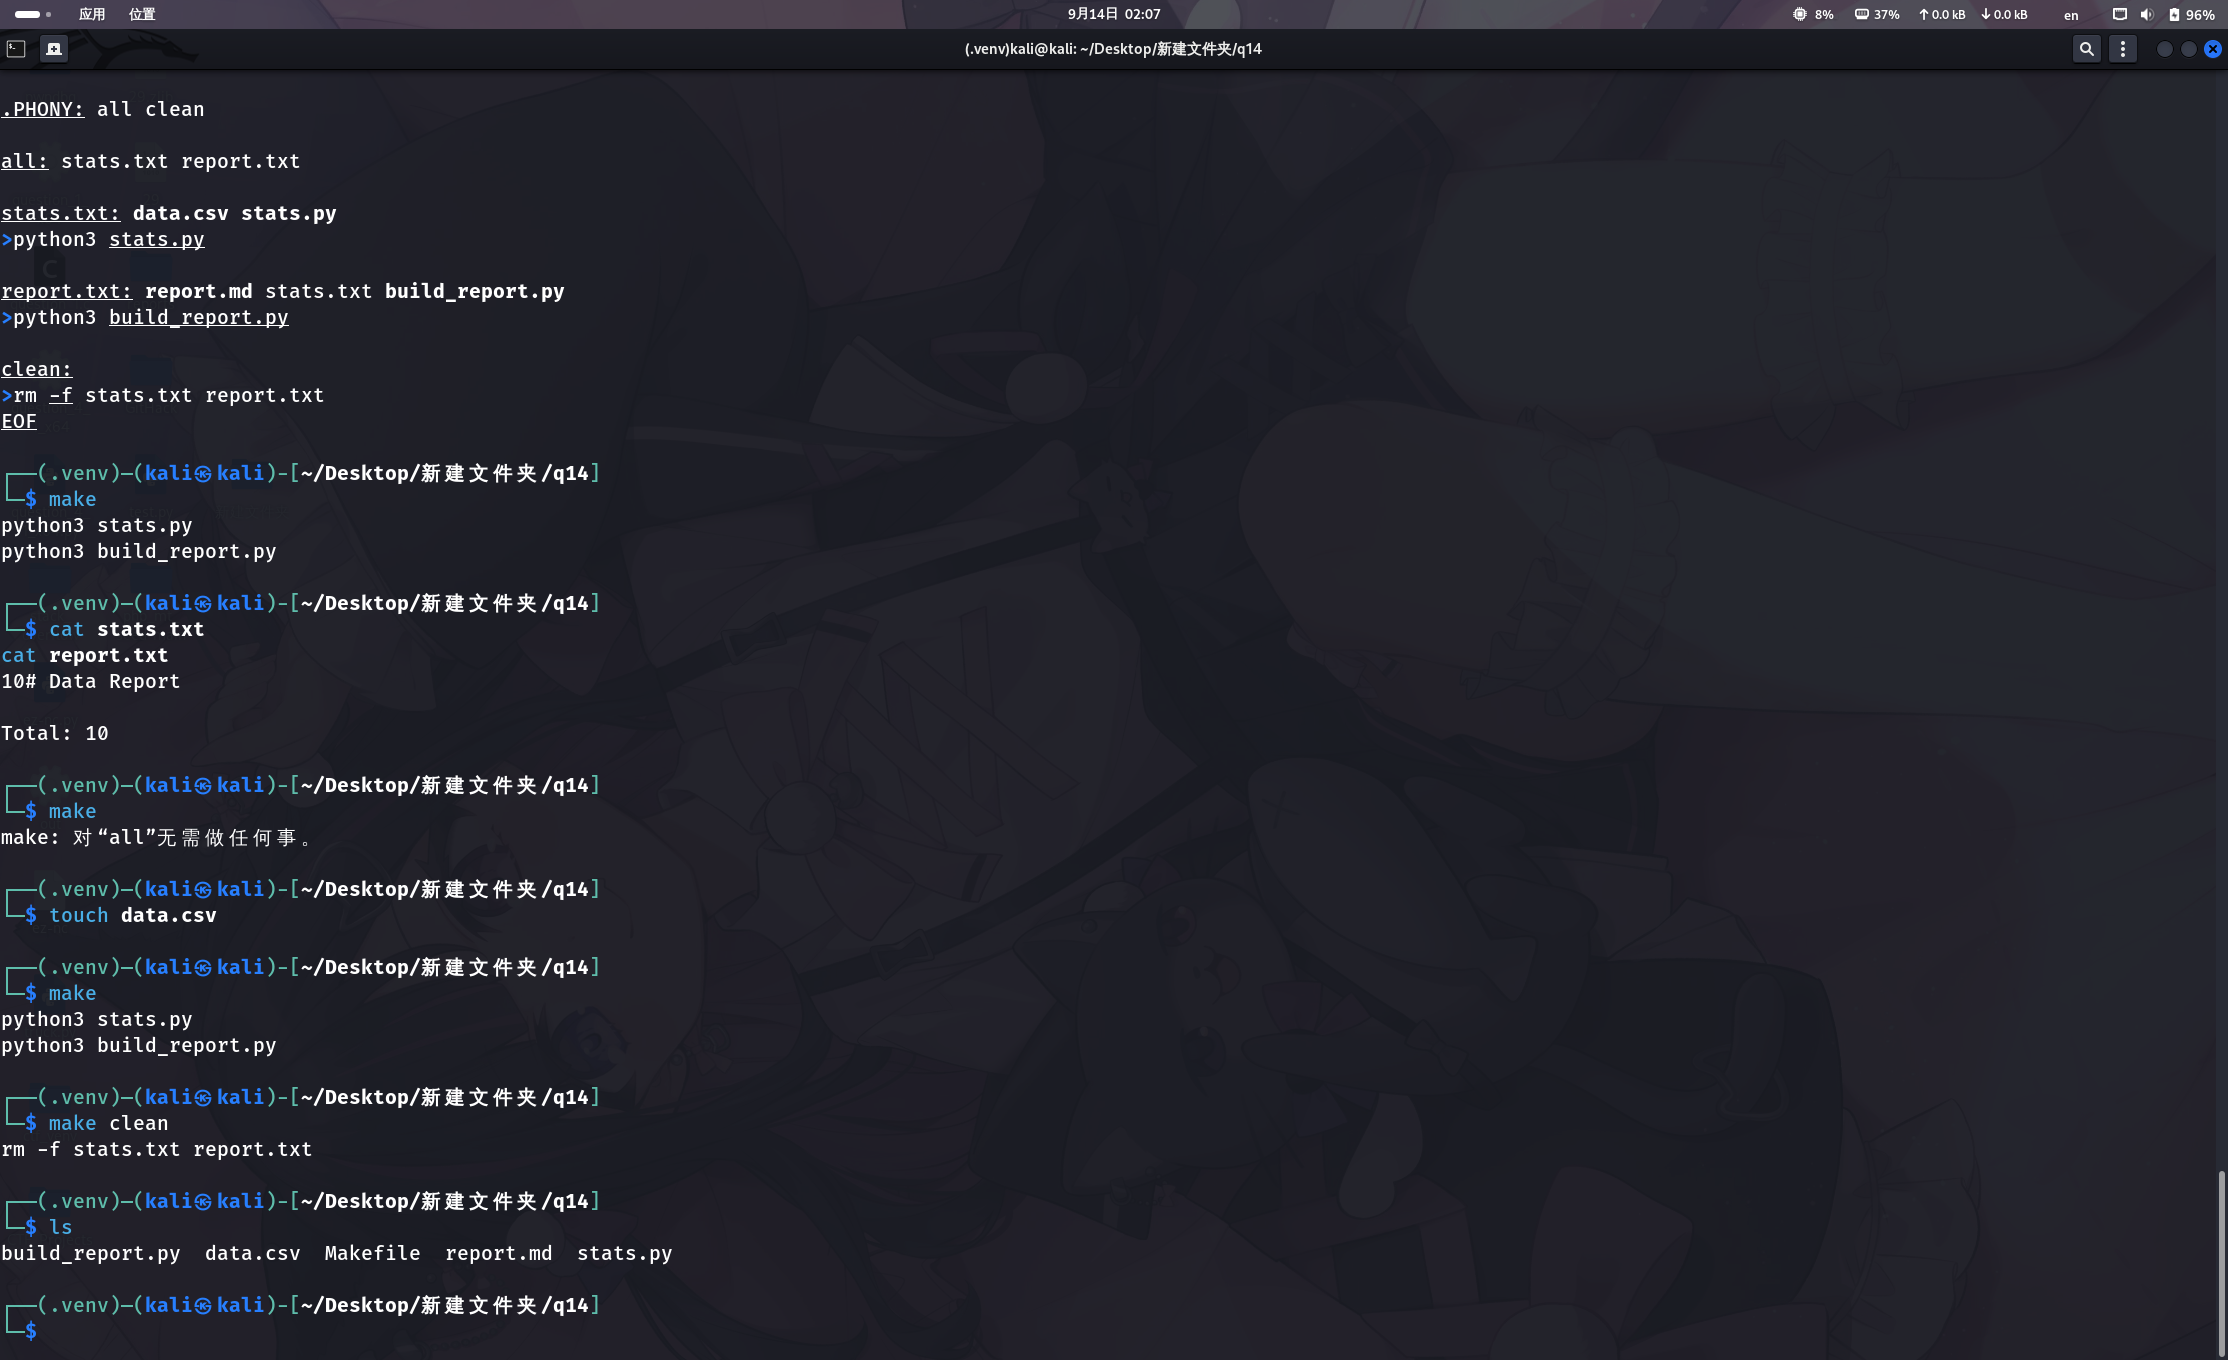
\includegraphics[width=.94\textwidth,height=.58\textheight,keepaspectratio]{assets/q14-make.png}
\caption{q14 的首次构建、增量构建与 clean 验证}
\end{figure}
\begin{summarybox}{结果说明}统计结果为 10，报告正确写入 \texttt{Total: 10}。第二次构建提示目标无需重建；\texttt{touch data.csv} 后两个 Python 脚本均再次执行；\texttt{clean} 后仅保留四个源文件和 Makefile。\end{summarybox}

\clearpage\exercisebanner{15}{把本地 API 数据转换为可读报告}{curl 与 jq}
\subsection*{执行内容}
在 q15 中通过 \texttt{python3 -m http.server 8000} 提供 \texttt{packages.json}，\texttt{api\_report.sh} 使用 curl 获取 JSON，再由 jq 过滤 \texttt{active} 且下载量不少于 100 的记录，并按下载量降序、名称升序输出 Markdown 表格。
\begin{lstlisting}[style=shell]
python3 -m http.server 8000 > server.log 2>&1 &
server_pid=$!
sleep 1
./api_report.sh
cat summary.md
kill "$server_pid"
\end{lstlisting}
\begin{figure}[H]\centering
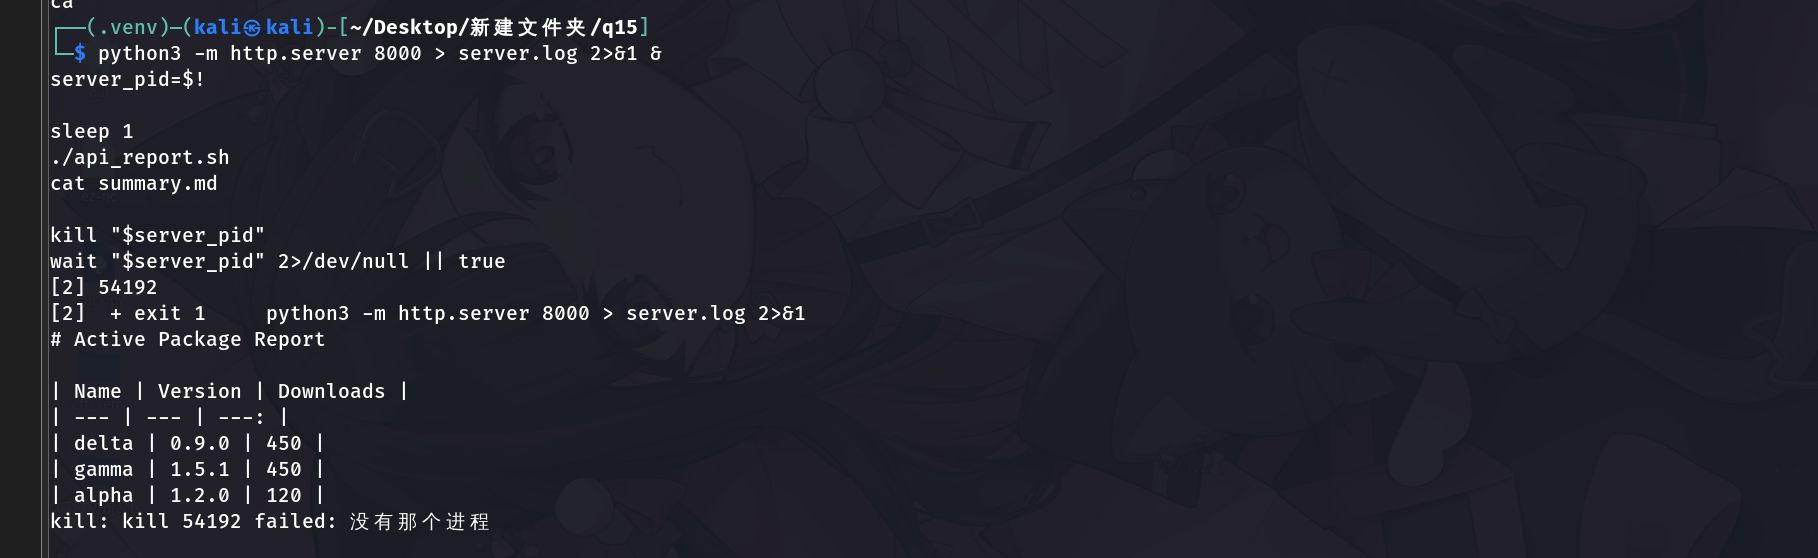
\includegraphics[width=.94\textwidth,height=.48\textheight,keepaspectratio]{assets/q15-report.png}
\caption{q15 生成的活动软件包 Markdown 报告}
\end{figure}
\begin{summarybox}{结果说明}生成的表格包含 delta、gamma 和 alpha 三条记录，下载量分别为 450、450、120。两个 450 下载量记录按名称升序排列，符合排序要求。服务进程已结束时再次 kill 的提示不影响报告生成。\end{summarybox}

\clearpage\exercisebanner{16}{修复并交付陌生的小型工具包}{测试、构建与 Git}
\subsection*{执行内容}
q16 从 q13 复制，并初始化独立 Git 仓库。先将问候实现临时改为固定输出 \texttt{Hello, name!}，再以 \texttt{make check} 验证正常姓名测试会失败；随后恢复使用传入姓名的实现，重新检查并构建 wheel。
\begin{lstlisting}[style=shell]
make check                 # 故意错误时失败
make check                 # 修复后通过
make build
ls -lh dist/
git add .
git commit -m "feat: deliver verified greetlab package"
\end{lstlisting}
\begin{figure}[H]\centering
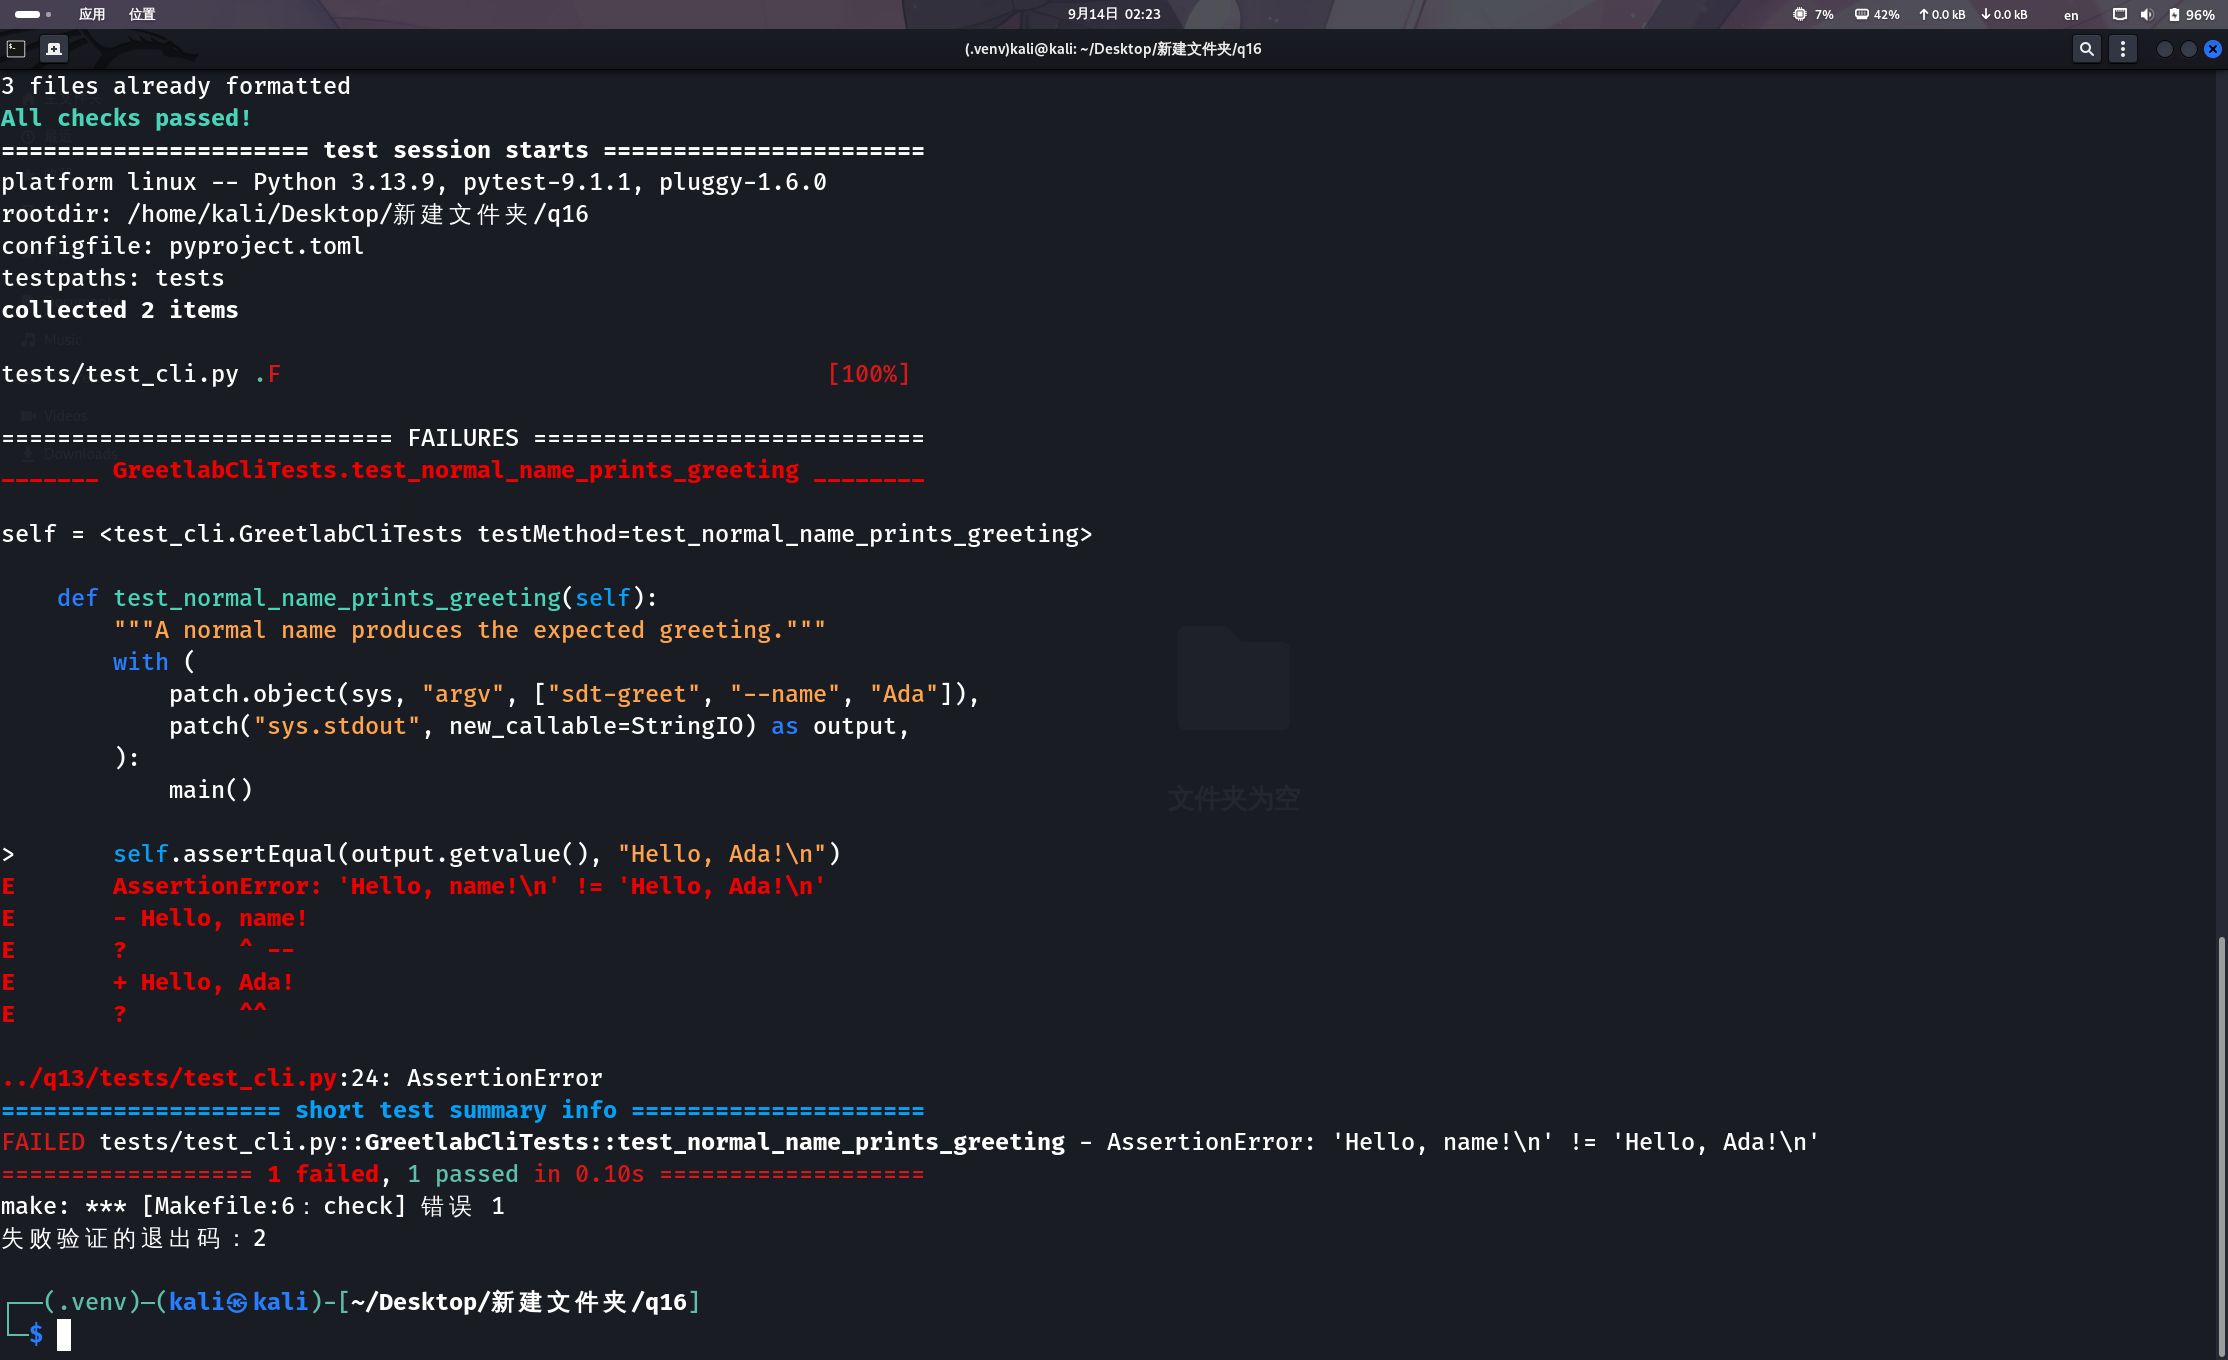
\includegraphics[width=.94\textwidth,height=.54\textheight,keepaspectratio]{assets/q16-failing-check.png}
\caption{q16 中固定问候语导致正常姓名测试失败}
\end{figure}
\begin{summarybox}{结果说明}失败时实际输出为 \texttt{Hello, name!}，与期望的 \texttt{Hello, Ada!} 不一致，\texttt{make check} 返回非零状态，说明测试能有效定位回归。\end{summarybox}

\clearpage\exercisebanner{16}{修复验证与交付}{测试、构建与 Git}
\begin{figure}[H]\centering
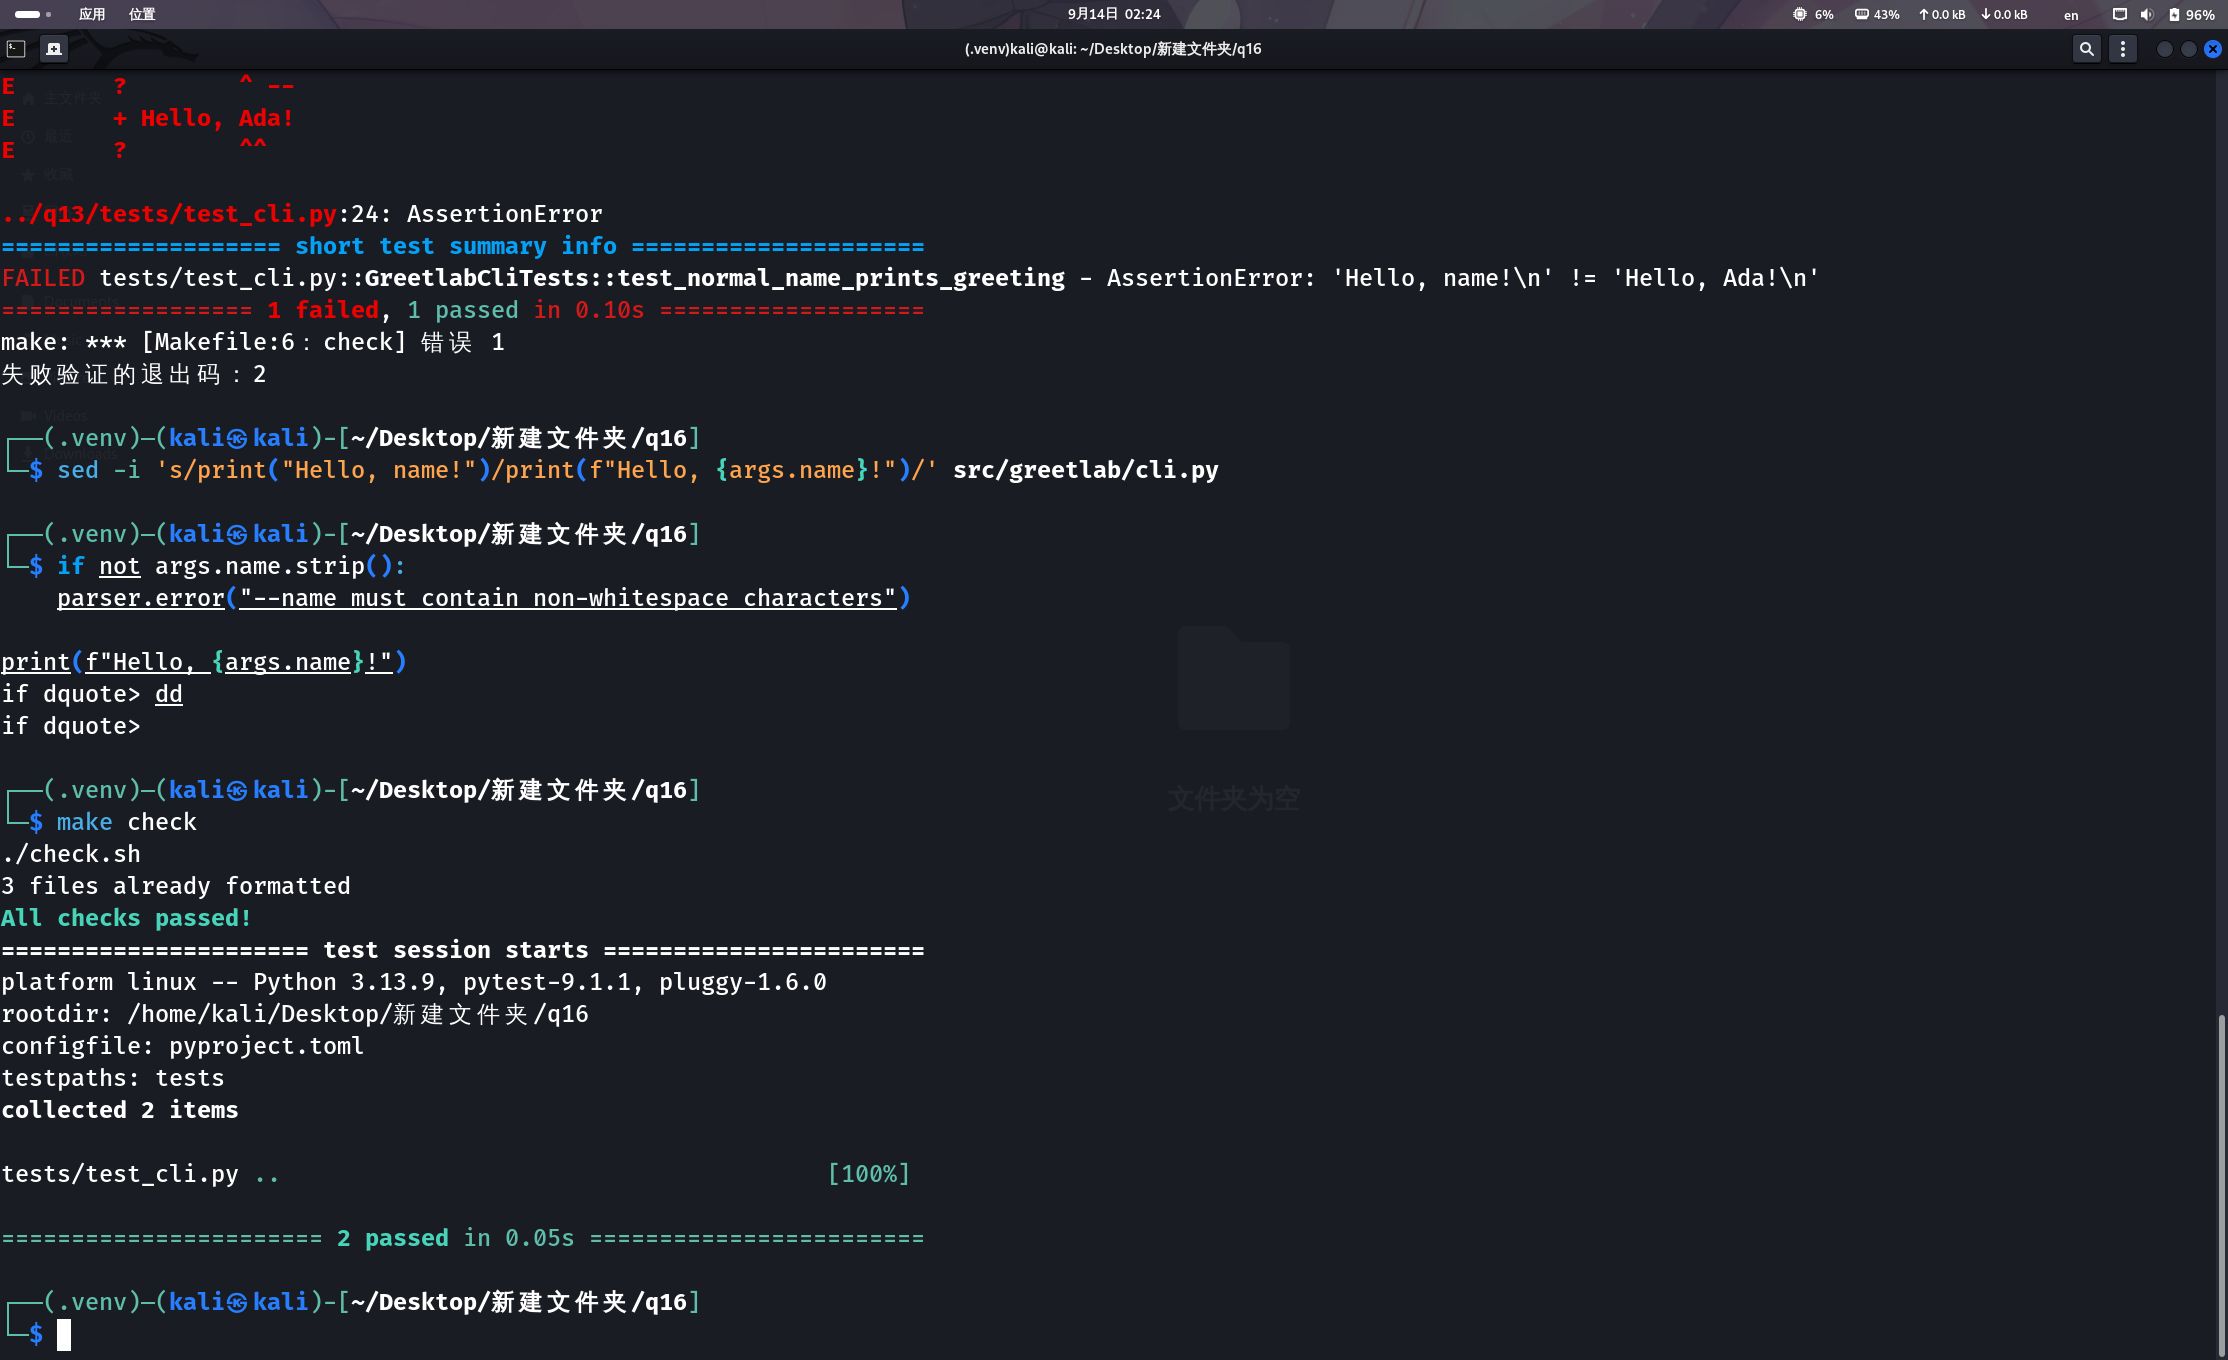
\includegraphics[width=.94\textwidth,height=.52\textheight,keepaspectratio]{assets/q16-passing-check.png}
\caption{q16 修复后 make check 通过}
\end{figure}
\begin{summarybox}{修复结果}恢复问候函数后，两项测试均通过，说明正常姓名与空白姓名两个行为均得到验证。\end{summarybox}
\clearpage
\begin{figure}[H]\centering
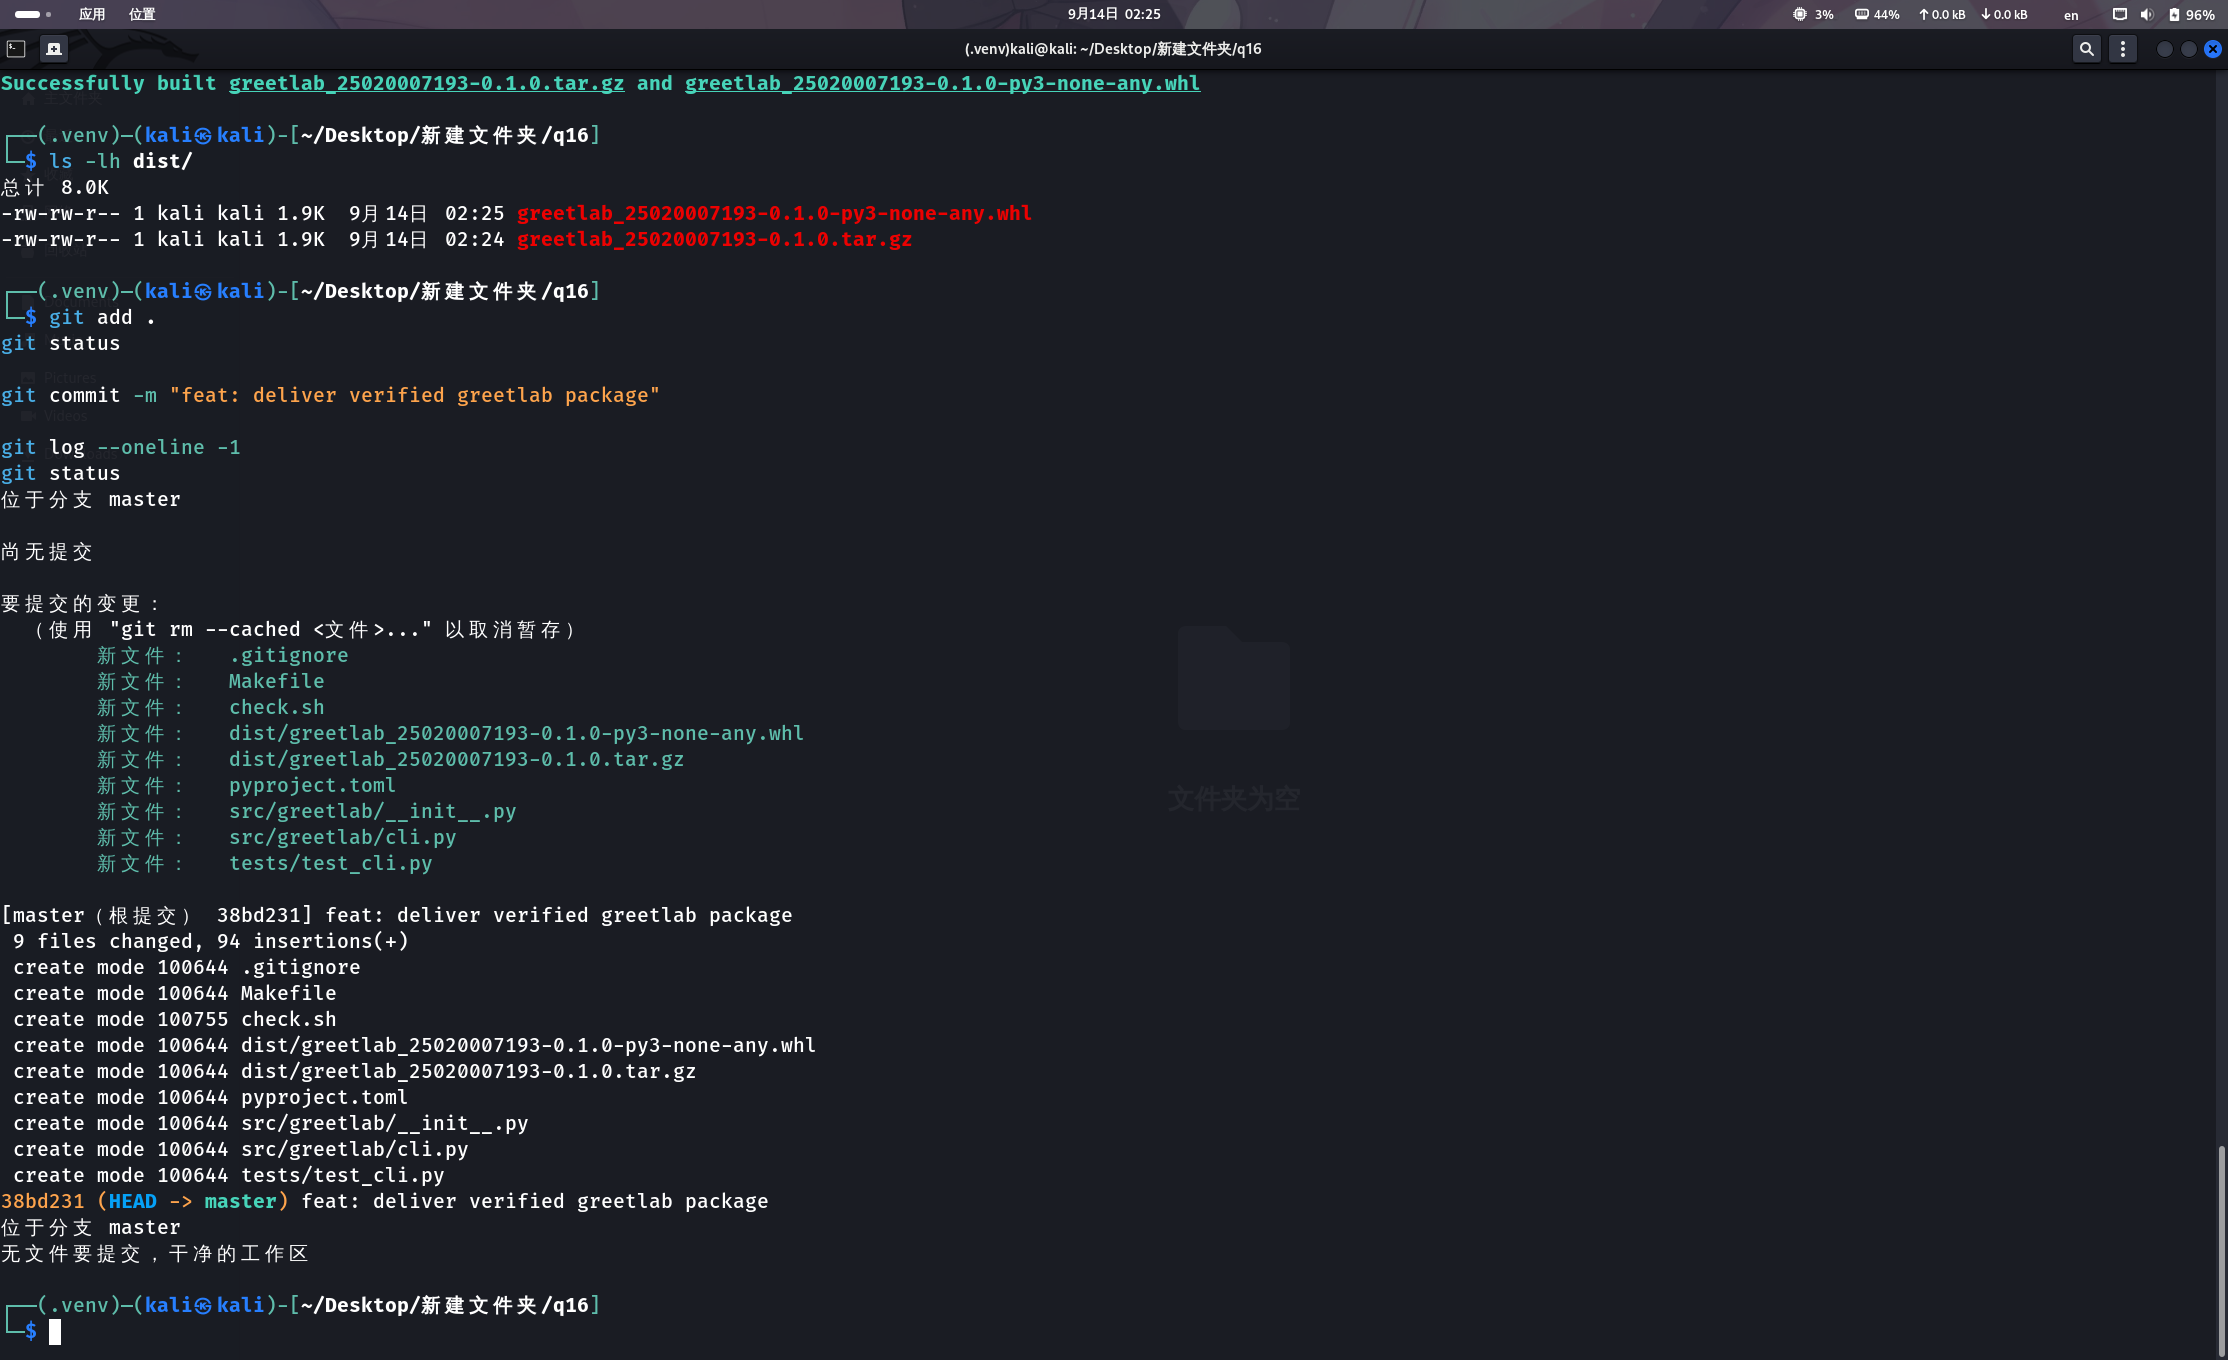
\includegraphics[width=.94\textwidth,height=.54\textheight,keepaspectratio]{assets/q16-build-git.png}
\caption{q16 成功构建 wheel 与 source distribution，并完成 Git 提交}
\end{figure}
\begin{summarybox}{交付结果}\texttt{make build} 成功生成 wheel 和源代码压缩包；Git 提交 \texttt{38bd231} 后的工作区状态为干净。\end{summarybox}

\clearpage\exercisebanner{1}{配置格式化器并验证只检查模式}{格式化}
\subsection*{任务与执行命令}
对项目中的不规范 Python 文件先运行检查，随后格式化并复查。\begin{lstlisting}[style=shell]
python -m ruff format --check src tests
python -m ruff format src tests
python -m ruff format --check src tests
\end{lstlisting}
\begin{summarybox}{结果说明}首次检查发现格式差异；格式化命令仅调整空格、引号和换行等表层风格；最终只检查模式返回 0。这符合 CI 中“检查而不修改文件”的原则。\end{summarybox}
\clearpage\exercisebanner{2}{用 linter 捕获未使用导入}{Lint}
\subsection*{任务与执行命令}
在示例模块故意保留 \texttt{import os}，验证静态分析后使用自动修复。\begin{lstlisting}[style=shell]
python -m ruff check src
python -m ruff check src --fix
python -m ruff check src
\end{lstlisting}
\begin{summarybox}{结果说明}Ruff 在不运行程序的前提下报告 F401（未使用的导入）。自动修复删除该导入，最终检查通过；修复后仍应人工审阅差异。\end{summarybox}
\clearpage\exercisebanner{3}{为问候函数编写单元测试}{测试}
\subsection*{任务与执行命令}
测试普通姓名、前后空格以及空白姓名拒绝三种行为。\begin{lstlisting}[style=shell]
pytest -q tests/test_greet.py
# 3 passed
\end{lstlisting}
\begin{summarybox}{结果说明}测试覆盖正常输入和非法输入。空白姓名必须抛出 \texttt{ValueError}，从而防止程序悄然生成无效问候语。\end{summarybox}
\clearpage\exercisebanner{4}{生成覆盖率报告并补足分支}{测试覆盖率}
\subsection*{任务与执行命令}\begin{lstlisting}[style=shell]
coverage run -m pytest
coverage report -m
coverage html
\end{lstlisting}
\begin{summarybox}{结果说明}补充空白姓名测试后，\texttt{greet.py} 的有效执行行均被运行。HTML 报告位于 \texttt{htmlcov/index.html}；覆盖率用于发现遗漏路径，不能替代对断言质量的判断。\end{summarybox}
\clearpage\exercisebanner{5}{配置 pre-commit 质量门禁}{Pre-commit 钩子}
\subsection*{任务与执行命令}\begin{lstlisting}[style=shell]
pre-commit install
pre-commit run --all-files
git commit -m "chore: enable quality checks"
\end{lstlisting}
\begin{summarybox}{结果说明}配置文件使提交前自动执行 Ruff 格式检查、Ruff lint 与 pytest。若其中任一项失败，提交会被阻止，先修复再提交。\end{summarybox}
\clearpage\exercisebanner{6}{为 push 配置持续集成}{持续集成}
\subsection*{任务与执行命令}\begin{lstlisting}[style=shell]
git add .github/workflows/quality.yml
git commit -m "ci: verify format lint and tests"
git push
\end{lstlisting}
\begin{summarybox}{结果说明}工作流在 \texttt{push} 与 \texttt{pull\_request} 时使用独立的 Ubuntu 环境安装依赖，并依次执行格式检查、lint 和测试。本地修改造成的 lint 错误应使 CI 失败。\end{summarybox}
\clearpage\exercisebanner{7}{通过 Makefile 统一命令入口}{命令运行器}
\subsection*{任务与执行命令}\begin{lstlisting}[style=shell]
make format-check
make lint
make test
make check
\end{lstlisting}
\begin{summarybox}{结果说明}开发者只需记住简短、稳定的 \texttt{make} 目标；底层工具参数集中在 Makefile 中。\texttt{check} 汇总所有质量检查，并在任一步失败时返回非零状态。\end{summarybox}
\clearpage\exercisebanner{8}{用正则查找危险 shell=True 调用}{正则表达式}
\subsection*{任务与执行命令}\begin{lstlisting}[style=shell]
grep -RInE 'subprocess\.Popen\([^)]*shell[[:space:]]*=[[:space:]]*True' .
# semgrep -l python -e 'subprocess.Popen(..., shell=True, ...)' .
\end{lstlisting}
\begin{summarybox}{结果说明}grep 能找出同一行内的常见写法；若参数分行、顺序变化或代码结构更复杂，纯文本模式可能漏报。语义工具 semgrep 更适合执行可维护的安全规则。\end{summarybox}
\clearpage\exercisebanner{9}{精确替换 Markdown 项目符号}{正则查找替换}
\subsection*{任务与执行命令}\begin{lstlisting}[style=shell]
python -c "import re,pathlib; p=pathlib.Path('notes.md'); s=p.read_text(); p.write_text(re.sub(r'(?m)^- (?=\\S)', '* ', s))"
\end{lstlisting}
\begin{summarybox}{结果说明}模式锚定行首，仅替换 Markdown 列表标记 \texttt{- }；日期、减号和正文中的连字符不会被误改。替换前后应使用 \texttt{git diff} 审阅。\end{summarybox}
\clearpage\exercisebanner{10}{从 JSON 提取 name，并比较两种方案}{正则与解析器}
\subsection*{任务与执行命令}\begin{lstlisting}[style=shell]
python extract_name.py < person.json
python -c "import re; print(re.search(r'\"name\"\s*:\s*\"((?:\\\\.|[^\"])*)\"', open('person.json').read()).group(1))"
\end{lstlisting}
\begin{summarybox}{结果说明}非贪婪或转义感知的 regex 可用于受控示例；正式 JSON 应使用 \texttt{json.load}，因为它能正确处理转义、字段顺序、嵌套结构和格式变化。\end{summarybox}
\vspace{.7cm}\begin{summarybox}{解题感悟}代码质量不是单一工具的结果，而是格式化、静态检查、测试、构建和版本控制门禁的组合。正则表达式适合明确的小范围匹配；面对结构化数据，应优先使用对应解析器。\end{summarybox}
\vspace{.55cm}\begin{summarybox}{参考资料}\centering\url{https://missing-semester-cn.github.io/2026/code-quality/}\end{summarybox}
\end{document}
